\begin{frame}
    \frametitle{Outline} 
    \tableofcontents[currentsection]
\end{frame} 

\begin{frame}
    \frametitle{Original Boxmodel Setup}

    \vspace{-0.5cm}
    \begin{itemize}
        \item MECCA boxmodel over 7 days. \vspace{6mm}
        \item Initial NMVOC typical of Los Angeles. \vspace{6mm}
        \item NO source tuned for maximum \ce{O3} production. 
    \end{itemize}
\end{frame}

\begin{frame}
    \frametitle{Original Boxmodel Setup (cont.)}

    \vspace{-5mm}
    \begin{itemize}
        \item Tagging follows organic products from VOC degradation \\ \hspace{2mm}$\Rightarrow$ effects on \ce{O3} production inferred from \ce{O_x} production. \vspace{4mm}
        \item Constant PBL height of 1 km \\ \hspace{2mm}$\Rightarrow$ no vertical mixing. \vspace{4mm}
        \item Constant temperature of 293 K.
    \end{itemize}
\end{frame}

\begin{frame}
    \frametitle{1. Tagging Approach}

    \vspace{-5mm}
    \begin{itemize}
        \item VOC tagging approach implemented in global model \\ by Shuai and Tim. \vspace{3mm}
        \item Allows allocation of \ce{O3} mixing ratios to source rather than comparing \ce{O_x} production. \vspace{3mm}
        \item Tagged MOZART-4 mechanism that was implemented in boxmodel for mechanism comparison study.
    \end{itemize}
\end{frame}

{
    \usebackgroundtemplate{%
        \vbox to \paperheight{\vfil\hbox to \paperwidth{\hfil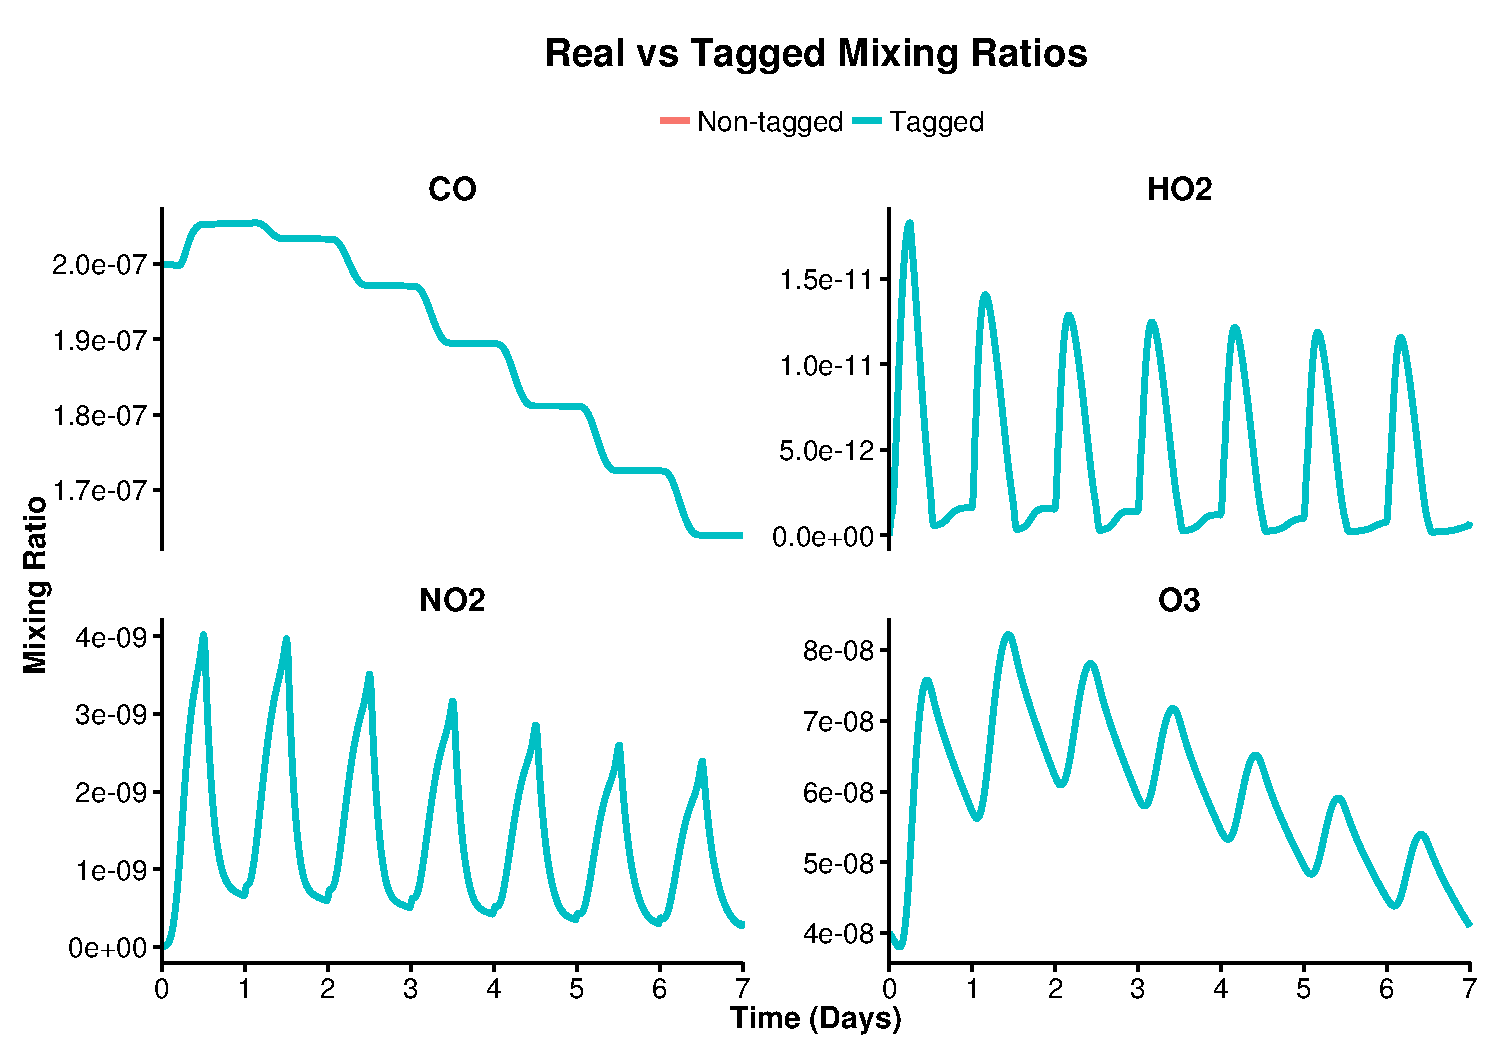
\includegraphics[height=0.90\paperheight, width = 0.98\paperwidth]{../Plotting_scripts/tagged_non-tagged_mixing_ratios}\hfil}\vfil}
    }
    \begin{frame}[plain]
    \end{frame}
}

{
    \usebackgroundtemplate{%
        \vbox to \paperheight{\vfil\hbox to \paperwidth{\hfil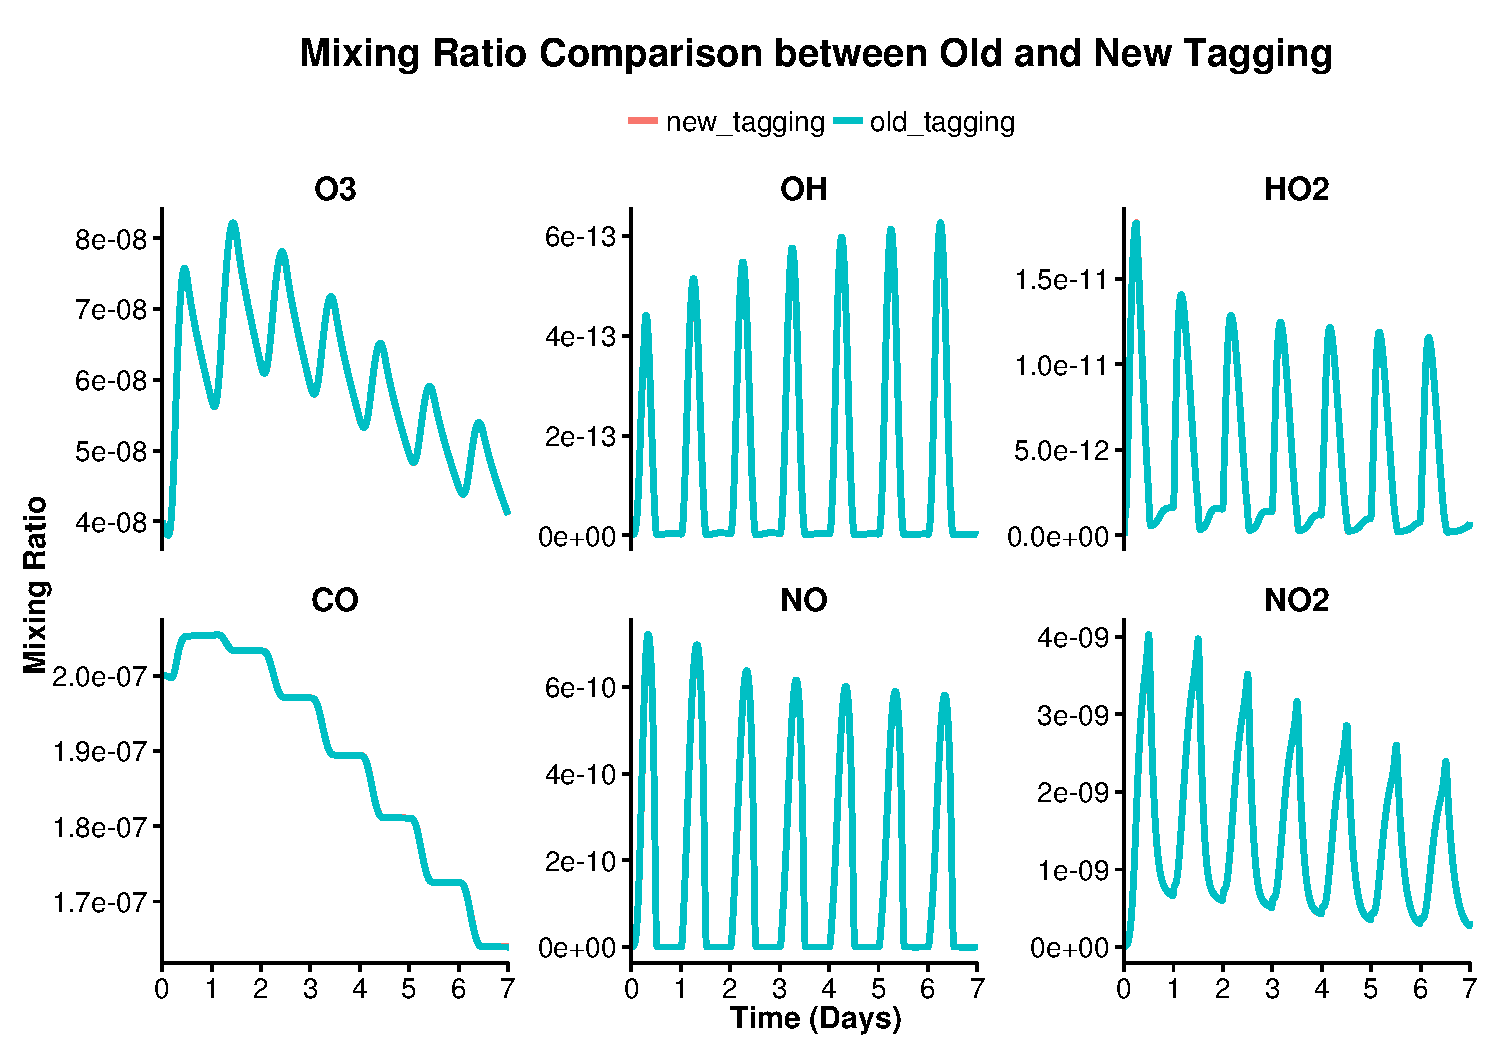
\includegraphics[height=0.90\paperheight, width = 0.98\paperwidth]{../Plotting_scripts/old_vs_new_tagging_mixing_ratios}\hfil}\vfil}
    }
    \begin{frame}[plain]
    \end{frame}
}

{
    \usebackgroundtemplate{%
        \vbox to \paperheight{\vfil\hbox to \paperwidth{\hfil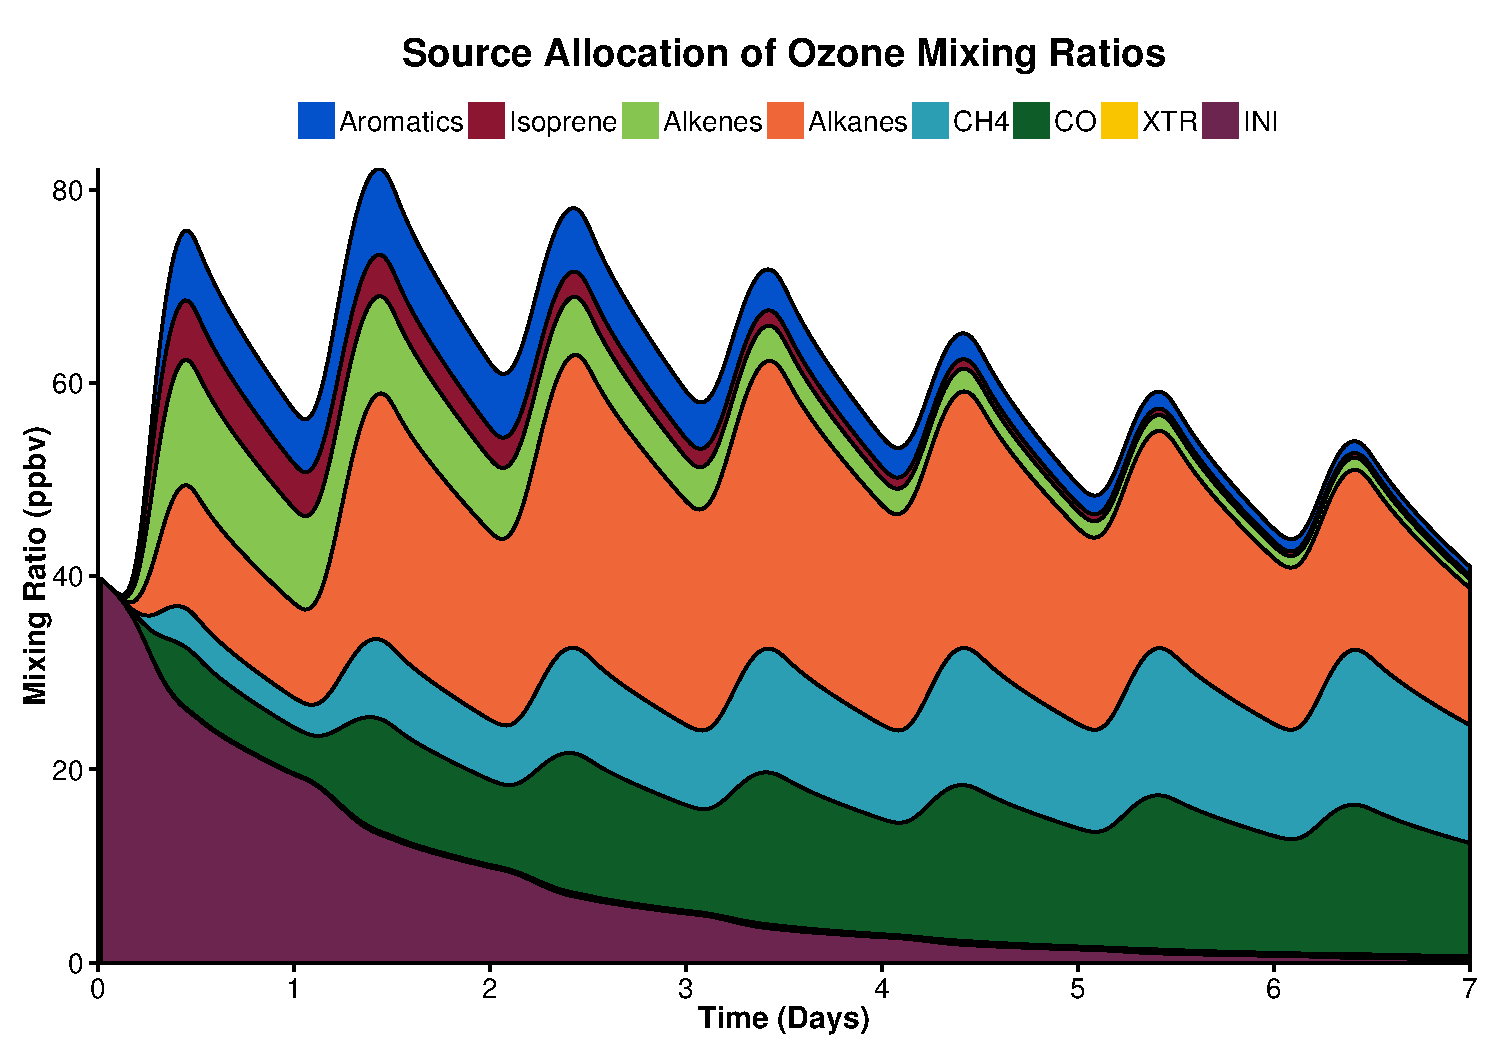
\includegraphics[height=0.90\paperheight, width = 0.98\paperwidth]{../Plotting_scripts/O3_mixing_ratio_components}\hfil}\vfil}
    }
    \begin{frame}[plain]
    \end{frame}
}

\begin{frame}
    \frametitle{2. Low and High \ce{NO_x} Conditions}

    \vspace{-5mm}
    \begin{itemize}
        \item Modelling rural and polluted urban conditions. \vspace{5mm}
        \item MOZART-4 mechanism with VOC tagging approach. \vspace{5mm}
        \item NO emissions calculated for maximum \ce{O3} production scaled 
            \begin{itemize}
                \item 0.5 for Low \ce{NO_x}
                \item 1.5 for High \ce{NO_x}
            \end{itemize}
    \end{itemize}
\end{frame}

{
    \usebackgroundtemplate{%
        \vbox to \paperheight{\vfil\hbox to \paperwidth{\hfil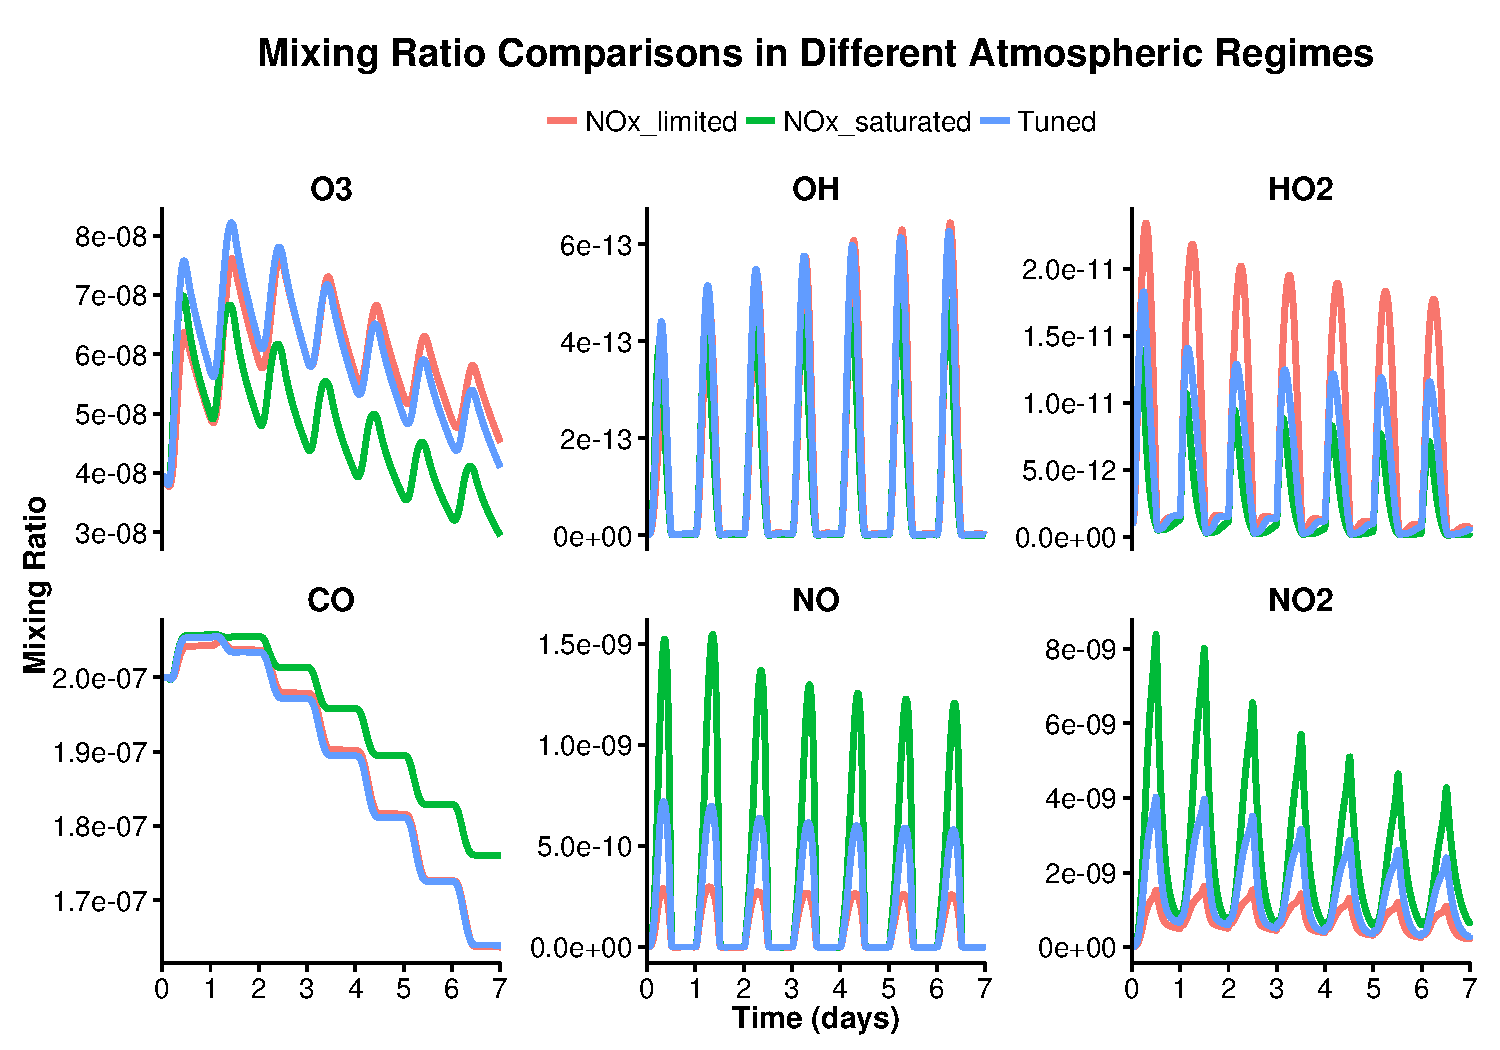
\includegraphics[height=0.90\paperheight, width = 0.98\paperwidth]{../Plotting_scripts/low_high_nox_non-tagged_mixing_ratios_comparison}\hfil}\vfil}
    }
    \begin{frame}[plain]
    \end{frame}
}

{
    \usebackgroundtemplate{%
        \vbox to \paperheight{\vfil\hbox to \paperwidth{\hfil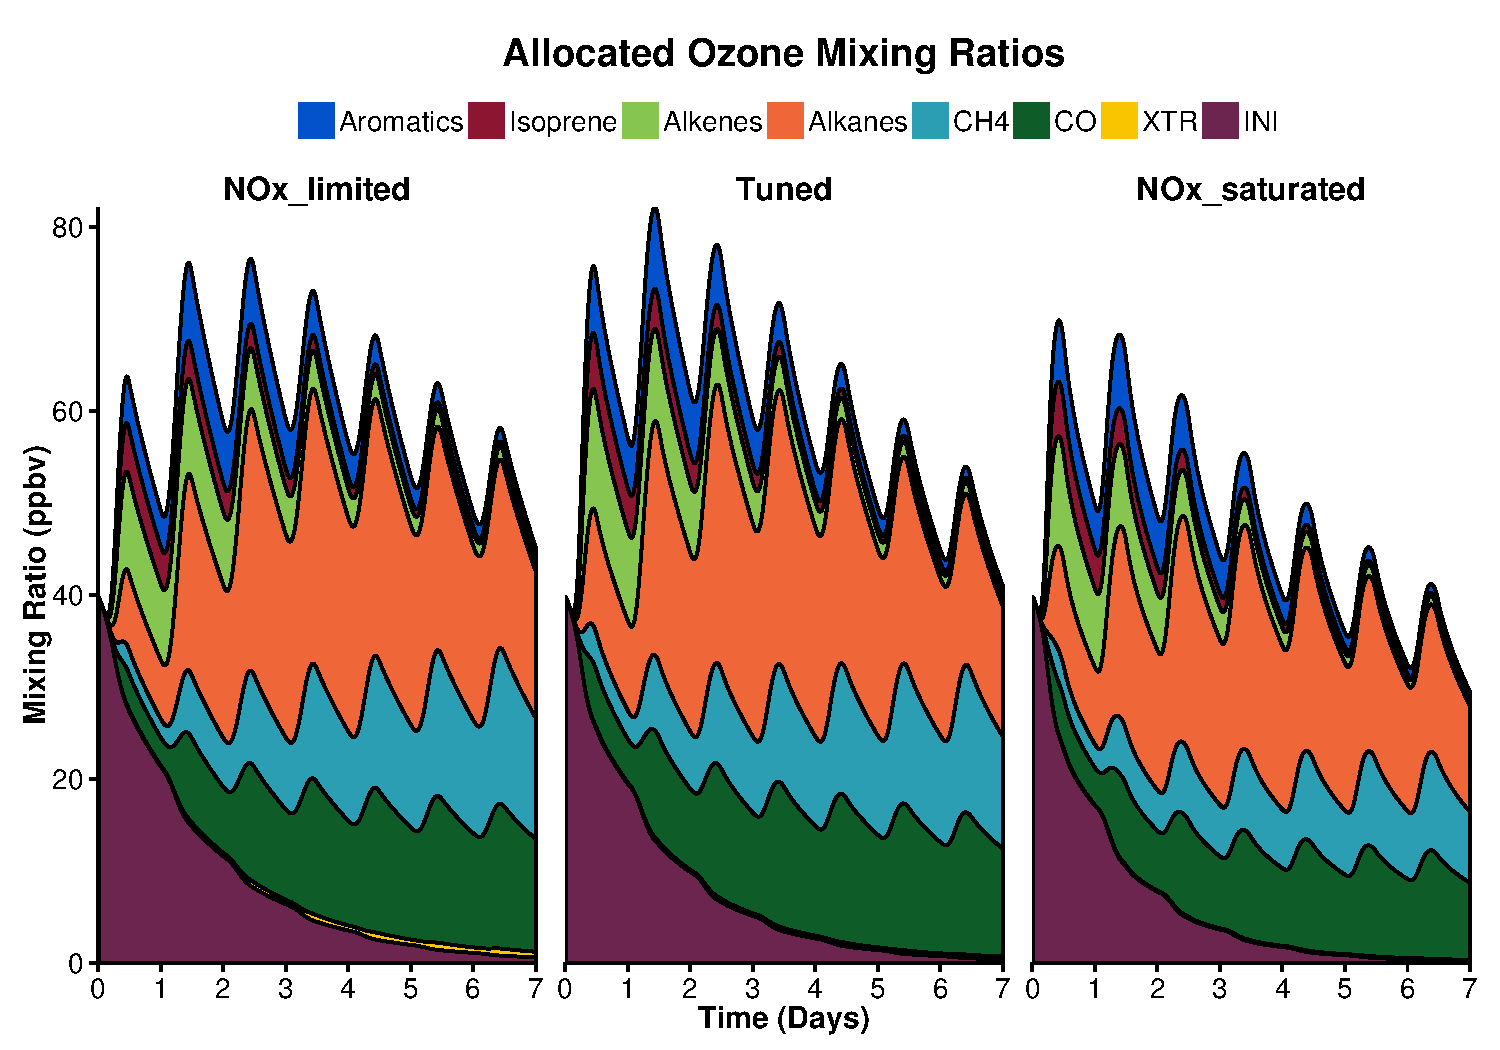
\includegraphics[height=0.90\paperheight, width = 0.98\paperwidth]{../Plotting_scripts/low_high_nox_O3_mixing_ratio_components_facet_run}\hfil}\vfil}
    }
    \begin{frame}[plain]
    \end{frame}
}

\begin{frame}
    \frametitle{3. Vertical Mixing}

    \vspace{-5mm}
    \begin{itemize}
        \item Included diurnal cycle for PBL height from CARES measurement campaign. \vspace{5mm}
        \item Vertical mixing with free troposphere approach from \\ Sandra Louren's thesis. \vspace{5mm}
        \item Free troposphere mixing ratios for \ce{O3} and CO from MATCH-MPIC model. 
    \end{itemize}
\end{frame}

{
    \usebackgroundtemplate{%
        \vbox to \paperheight{\vfil\hbox to \paperwidth{\hfil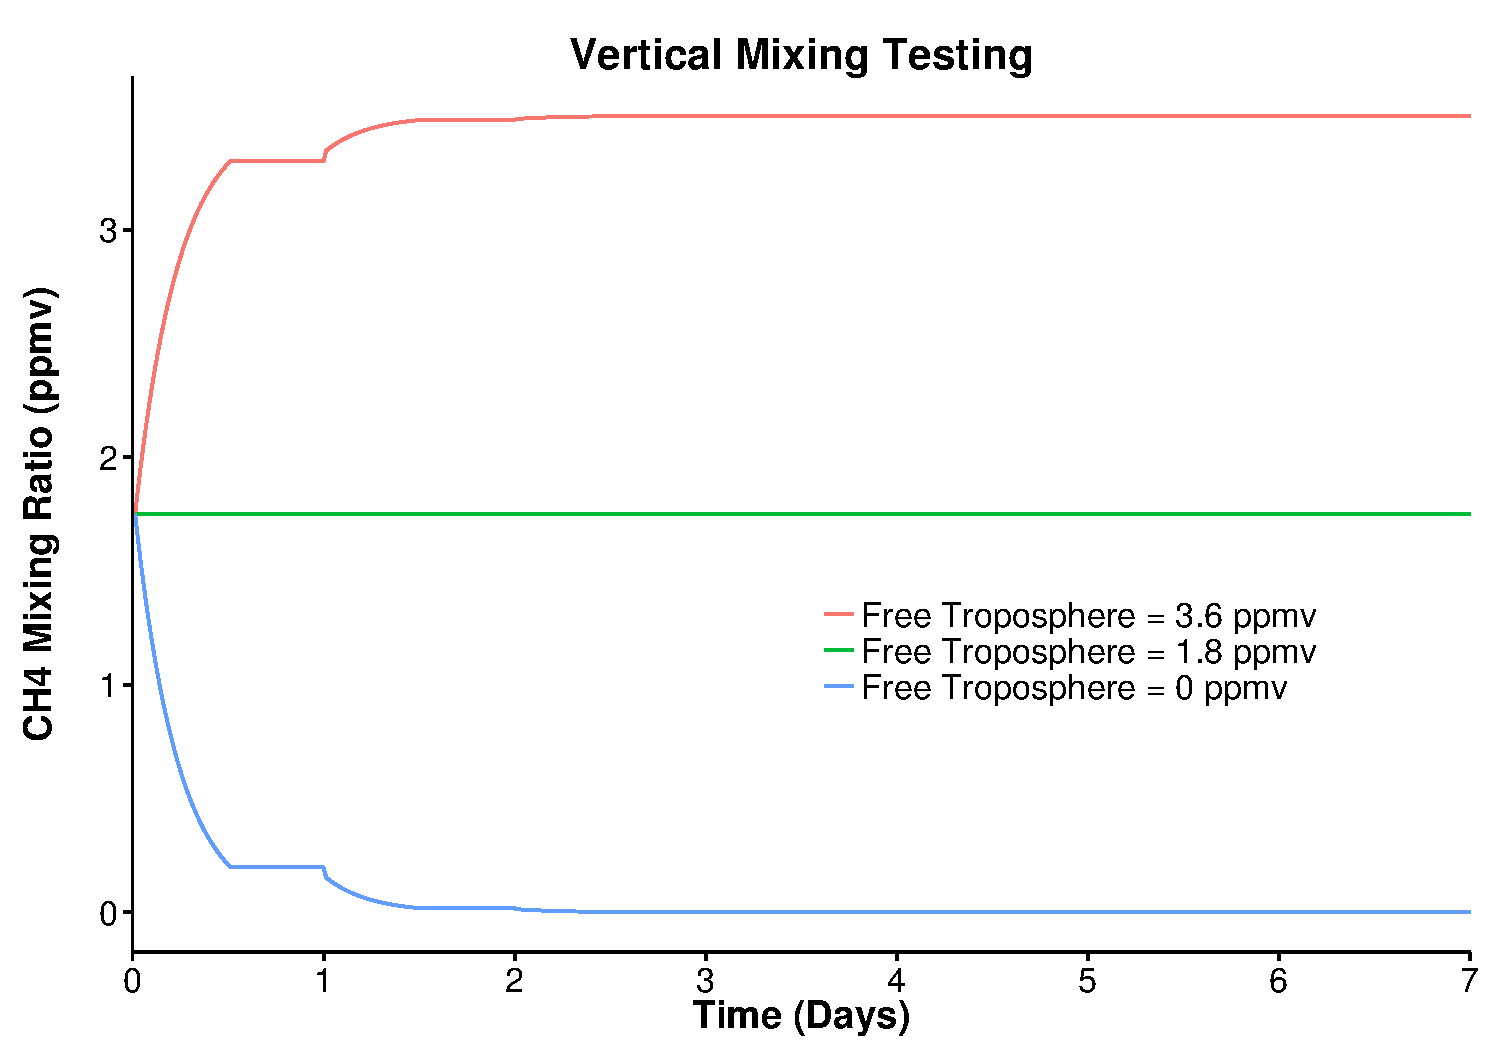
\includegraphics[height=0.98\paperheight, width = 0.98\paperwidth]{../Plotting_scripts/CH4_comparison_vertical_mixing}\hfil}\vfil}
    }
    \begin{frame}[plain]
    \end{frame}
}

{
    \usebackgroundtemplate{%
        \vbox to \paperheight{\vfil\hbox to \paperwidth{\hfil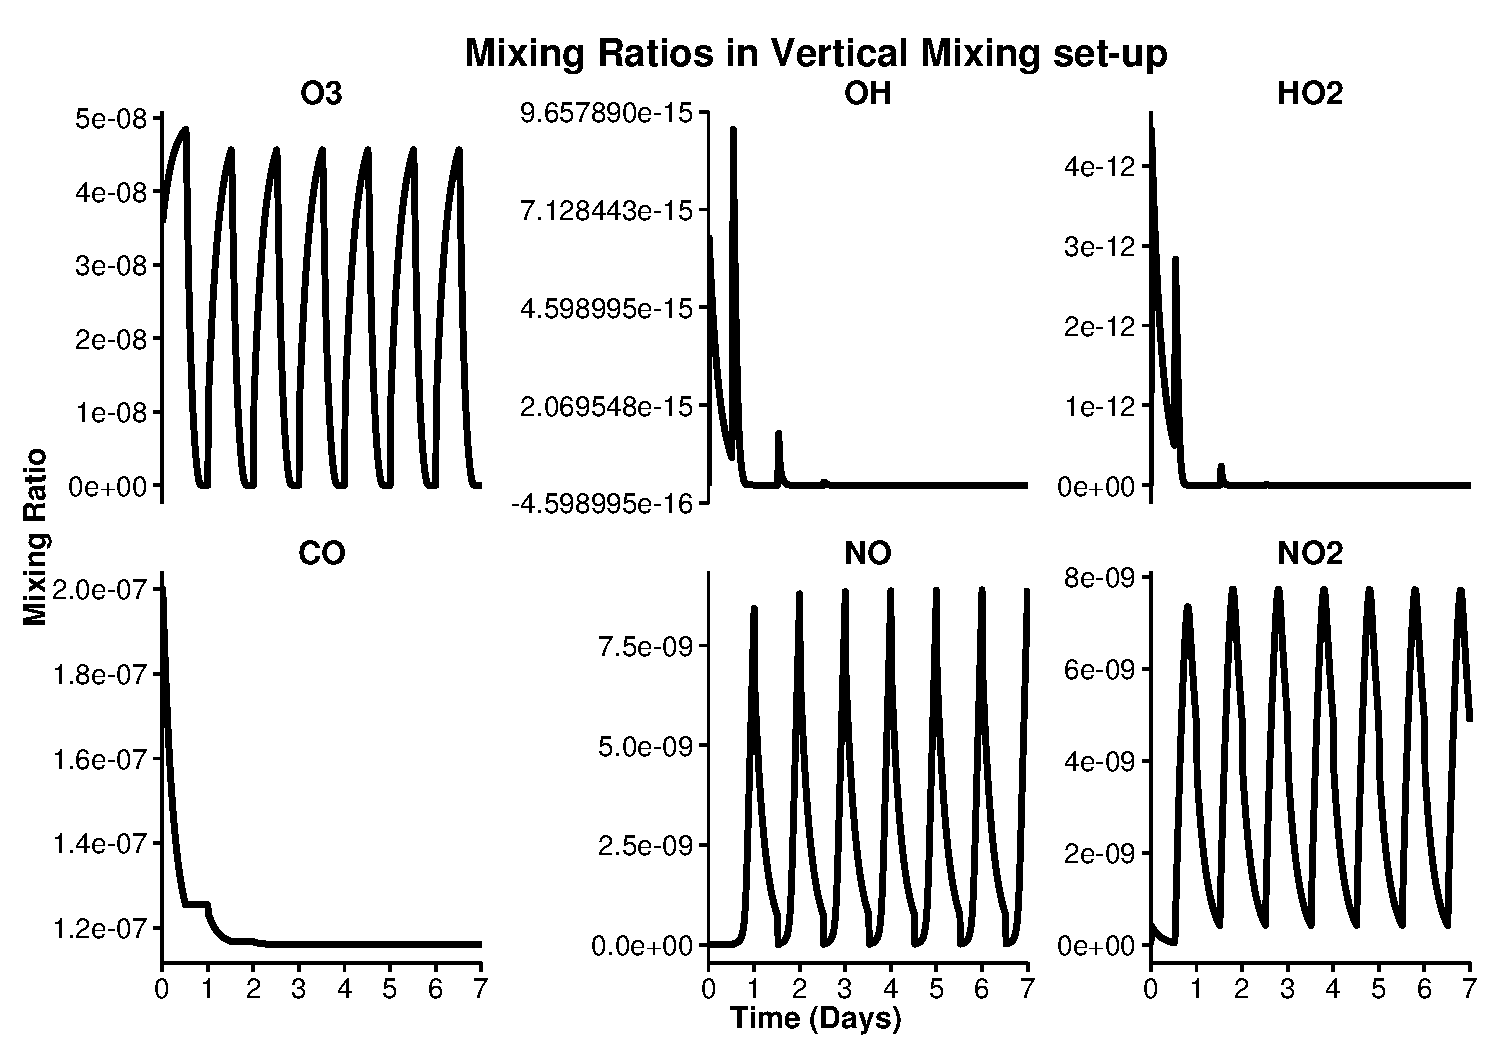
\includegraphics[height=0.90\paperheight, width = 0.98\paperwidth]{../Plotting_scripts/vertical_mixing_mixing_ratios}\hfil}\vfil}
    }
    \begin{frame}[plain]
    \end{frame}
}

%\begin{frame}
%    \frametitle{4. Horizontal Mixing}
%
%    \begin{itemize}
%        \item Same boxmodel set-up as VOC tagging approach.
%        \item Implement horizontal mixing approach as in Sandra Louren's thesis.
%        \item ??? what is the modelling case?
%    \end{itemize}
%\end{frame}

\begin{frame}
    \frametitle{4. Temperature}

    \vspace{-5mm}
    \begin{itemize}
        \item Run boxmodel at 295 K, scenario of a warmer climate. \vspace{3mm}
        \item Compare \ce{O3} between lower and higher temperatures. \vspace{3mm}
        \item According to recent review by Pusede et al., temperature dependent chemistry of alkyl nitrates impacts \ce{O3} production. \vspace{3mm}
        \item Assess how this chemistry is represented in the chemical mechanisms used in comparison study. 
    \end{itemize}
\end{frame}
